\documentclass[xcolor=dvipsnames]{beamer}
%\documentclass[aspectratio=169,xcolor=dvipsnames]{beamer}

%=================================================================================
% Document information
\def\firstname{Marc}
\def\familyname{Henry de Frahan}
\def\FileAuthor{\firstname~\familyname}
\def\FileTitle{ParCFD 2017}
\def\FileSubject{ParCFD 2017}
\def\FileKeyWords{\firstname~\familyname, \FileSubject, \FileTitle}

%=================================================================================
% Preamble
%=================================================================================
% PACKAGES
\usepackage{amsmath}
\usepackage{amssymb}
\usepackage{amsfonts}
\usepackage{wasysym} % for circles
\usepackage{graphicx}
\usepackage[utf8]{inputenc}
%\usepackage[usenames,dvipsnames]{color}
\usepackage{textcomp}
\usepackage{alltt}
%\usepackage{subfigure}
\usepackage{latexsym}
\usepackage{eurosym}
\usepackage{verbatim}
\usepackage{epstopdf}         % if you want to use .eps and .jpeg in the same document (compile with pdflatex directly)
\usepackage{array}            % permet d'utiliser m{width} dans l'env tabular
\usepackage[english]{babel}
\usepackage{multirow}
\usepackage{algorithmic}
\usepackage{units}
\usepackage{nicefrac}
\usepackage{natbib} 
\usepackage{appendix}
%\usepackage{chapterbib}
\usepackage{booktabs}
\usepackage{pdfpages}        % to include pdf pages into the doc \includepdf[pages={1}]{myfile.pdf}
\usepackage{layout}          % then \layout in the document to get the layout numbers
\usepackage{hyperref}        % Hyper references for the document
\usepackage{subcaption}
\hypersetup{
  colorlinks=true,       % false: boxed links; true: colored links
  breaklinks=true,    % permet le retour à la ligne dans les liens trop longs
  linkcolor=black,       % color of internal links (red)
  citecolor=black,       % color of links to bibliography (green)
  filecolor=black,       % color of file links (magenta)
  urlcolor=black,        % color of external links (cyan)
  pdftitle={\FileTitle},
  pdfauthor={\FileAuthor},
  pdfsubject={\FileSubject},
  pdfkeywords={\FileKeyWords}}

% BEAMER specific
\mode<article>{\usepackage{fullpage}}
\mode<presentation>
{
  \usetheme{default}
  \usecolortheme{default} % beetle, lily, beaver
}
\usepackage{tikz}
\usepackage{mdwlist}
\usepackage{moreverb}
\usepackage{etex}   % this is a dodgy fix for using lpic: http://www.tex.ac.uk/cgi-bin/texfaq2html?label=noroom
\usepackage{lpic}
\usepackage[absolute,overlay]{textpos} % for absolute positioning on page
\setbeamertemplate{navigation symbols}{}
\setbeamertemplate{footline}{\leavevmode% 
  \hfill\hbox{% 
    \begin{beamercolorbox}[wd=1.0\paperwidth,ht=2.25ex,dp=1ex,left]{date in head/foot}% 
      \scriptsize \hspace*{1ex} \insertframenumber{} %
    \end{beamercolorbox}}% 
  \vskip0pt%
}
\beamertemplatetransparentcovereddynamic
\beamertemplateballitem
\beamertemplatesolidbuttons
\usefonttheme[onlymath]{serif}
\setbeamercovered{invisible} % http://tex.stackexchange.com/questions/53860/can-i-tell-beamer-that-uncover-should-be-invisible-not-merely-grayed-out


%=================================================================================
% Useful commands
\newcommand{\minimum}[1]{\mathop{\textrm{min}}_{#1}\,}
\newcommand{\maximum}[1]{\mathop{\textrm{max}}_{#1}\,}
\newcommand{\argmin}[1]{\mathop{\textrm{arg min}}_{#1}\,}
\newcommand{\dg}{\textsc{dg}}
\newcommand{\bs}{\boldsymbol}
\newcommand{\mbf}[1]{\mathbf{#1}}
\newcommand{\com}[1]{\textcolor{red}{#1}\marginpar{\textcolor{red}{\Large $/!\backslash$}}}
\newcommand{\pfrac}[2]{\frac{\partial#1}{\partial#2}}
\newcommand{\dpfrac}[2]{\dfrac{\partial#1}{\partial#2}}
\newcommand{\ufrac}[2]{\frac{\ud{}#1}{\ud{}#2}}
\newcommand{\dufrac}[2]{\dfrac{\ud{}#1}{\ud{}#2}}
\newcommand{\wt}[1]{\widetilde{#1}}
\newcommand{\ol}[1]{\overline{#1}}
\newcommand{\avg}[1]{\left\{\!\!\left\{#1\right\}\!\!\right\}}
\newcommand{\jmp}[1]{\left[\!\left[#1\right]\!\right]}
\newcommand{\hr}{\textsc{hr}}
\newcommand{\xjl}{x_{j-\nicefrac{1}{2}}}
\newcommand{\xjr}{x_{j+\nicefrac{1}{2}}}
\newcommand{\xRl}{x_{I-\nicefrac{1}{2}}}
\newcommand{\xRr}{x_{I+\nicefrac{1}{2}}}
\newcommand{\xLl}{x_{(I-1)-\nicefrac{1}{2}}}
\newcommand{\xLr}{x_{(I-1)+\nicefrac{1}{2}}}
\newcommand{\ud}{\,\mathrm{d}}
\newcommand{\dgm}{\textsc{dgm}}
\newcommand{\fem}{\textsc{fem}}
\newcommand{\fvm}{\textsc{fvm}}
\newcommand{\cpu}{\textsc{cpu}}
\newcommand{\gpu}{\textsc{gpu}}
\newcommand{\gpub}{\textsc{gpublas}}
\newcommand{\blas}{\textsc{blas}}
\newcommand{\cublas}{\textsc{cublas}}
\newcommand{\cuda}{\textsc{cuda}}
\newcommand{\pcpu}{$P_{\cpu{}}$}
\newcommand{\pgpu}{$P_{\gpu{}}$}
\newcommand{\pgpub}{$P_{\gpub{}}$}
\newcommand{\pcpuc}{\textcolor{red}{$P_{\cpu{}}$}}
\newcommand{\pgpuc}{\textcolor{olivegreen}{$P_{\gpu{}}$}}
\newcommand{\pgpubc}{\textcolor{blue}{$P_{\gpub{}}$}}
\newcommand{\bth}{$B_{\text{theo}}$}
\newcommand{\bpr}{$B_{\text{pract}}$}
\newcommand{\bcpu}{$B_{\text{\cpu{}}}$}
\newcommand{\bgpu}{$B_{\text{\gpu{}}}$}
\newcommand{\bgpub}{$B_{\text{\gpub{}}}$}
\newcommand{\e}[1]{\ensuremath{\times 10^{#1}}}
\newcommand{\tabcn}[1]{\multicolumn{1}{c}{\makebox[0.65cm]{\tiny #1}}} % for a tabular workaround
\renewcommand*{\thesubfigure}{}  % Gets rid of the subfigure counter!!
\newcommand{\alf}{Alfvén}
\newcommand{\els}{Elsässer}
% Needed for the title page:
\newcommand{\HRule}{\rule{\linewidth}{0.5mm}}
\renewcommand{\topfraction}{0.85}
\renewcommand{\textfraction}{0.1}
\renewcommand{\floatpagefraction}{0.75}
% Needed for the natbib bibliography style
%\newcommand*{\newblock}{}
%% \bibpunct[<optional>]{}{}{;}{}{}{} 
% To put a box around a figure
\setlength\fboxsep{0pt}
\setlength\fboxrule{0.5pt}
\def\CC{{C\nolinebreak[4]\hspace{-.05em}\raisebox{.4ex}{\tiny\bf ++}}}

% increase space in underbrace env (http://tex.stackexchange.com/questions/13843/vertical-spacing-with-underbrace-command)
\newcommand*\mystrut[1]{\vrule width0pt height0pt depth#1\relax}

% https://tex.stackexchange.com/questions/33401/a-version-of-colorbox-that-works-inside-math-environments
\newcommand{\highlight}[2][yellow]{\mathchoice%
  {\colorbox{#1}{$\displaystyle#2$}}%
  {\colorbox{#1}{$\textstyle#2$}}%
  {\colorbox{#1}{$\scriptstyle#2$}}%
  {\colorbox{#1}{$\scriptscriptstyle#2$}}}%

%=================================================================================
% Define some colors
\definecolor{violetred}{rgb}{0.78,0.08,0.52}
\definecolor{olivegreen}{rgb}{0.2,0.6,0.0}
\definecolor{darkgray}{rgb}{0.95,0.95,0.95}
\definecolor{mypurple}{rgb}{0.76,0.06,0.76}
\definecolor{greenyellow}{rgb}{0.76,0.76,0.06}
\definecolor{gold}{HTML}{FFD700} 
\definecolor{IMnumber}{HTML}{AFB9DB}

% From http://www.google.com/url?sa=t&rct=j&q=&esrc=s&source=web&cd=1&ved=0CFcQFjAA&url=http%3A%2F%2Fwww.perceptualedge.com%2Farticles%2Fvisual_business_intelligence%2Frules_for_using_color.pdf&ei=TioYUPL8GMPl0QHhqICQAQ&usg=AFQjCNGA9t1pGae49wQ0DVhaSNcAk6oLyA&sig2=QuA9D9nierTbqn3djCyyPQ
\definecolor{c1med}{HTML}{F15A60} % red
\definecolor{c2med}{HTML}{7AC36A} % green
\definecolor{c3med}{HTML}{5A9BD4} % blue
\definecolor{c4med}{HTML}{FAA75B} % orange
\definecolor{c5med}{HTML}{9E67AB} % purple
\definecolor{c6med}{HTML}{CE7058} % burgundy
\definecolor{c7med}{HTML}{D77FB4} % magenta
\definecolor{c8med}{HTML}{737373} % grey

\definecolor{c1brt}{HTML}{EE2E2F} % red     
\definecolor{c2brt}{HTML}{008C48} % green   
\definecolor{c3brt}{HTML}{185AA9} % blue    
\definecolor{c4brt}{HTML}{F47D23} % orange  
\definecolor{c5brt}{HTML}{662C91} % purple  
\definecolor{c6brt}{HTML}{A21D21} % burgundy
\definecolor{c7brt}{HTML}{B43894} % magenta 
\definecolor{c8brt}{HTML}{010202} % black

\newcommand{\tcb}[2]{\textcolor{c#1brt}{#2}}
\newcommand{\tcm}[2]{\textcolor{c#1med}{#2}}

%=================================================================================
% Tikz special stuff (do after color definitions)
\usetikzlibrary{decorations.pathreplacing}
\usetikzlibrary{calc}
\usetikzlibrary{decorations.shapes}
\usetikzlibrary{decorations.pathmorphing}
\tikzset{paint/.style={fill=red}, decorate with/.style={decorate,decoration={shape backgrounds,shape=#1,shape size=3pt}}}
\tikzset{dotr/.style={fill=c1brt,circle,minimum size=3pt}}
\tikzset{dotb/.style={fill=c3brt,circle,minimum size=3pt}}
\tikzset{dotrr/.style={fill=c1brt,circle,minimum size=0.2cm,inner sep=0}}
\usetikzlibrary{positioning}
\usetikzlibrary{shapes}
\usetikzlibrary{snakes}
%fill=red,circle,minimum size=3pt
\usepackage{pgfkeys}
\usepackage{pgf,pgfarrows,pgfnodes,pgfautomata,pgfheaps,pgfshade}

%=================================================================================
% Environments 
% Theorem environments (from http://www.math.uiuc.edu/~hildebr/tex/theorems.html)
\newtheorem{thm}{Théorème}[section]
\newtheorem{cor}[thm]{Corollary}
\newtheorem{lem}[thm]{Lemma}
%\theoremstyle{remark}
\newtheorem{rem}[thm]{Remark}
%\theoremstyle{definition}
%\newtheorem{def}[thm]{Definition}

% Tight lists
\newenvironment{tight-itemize}
{\begin{itemize}
  \setlength{\itemsep}{1pt}
  \setlength{\parskip}{0pt}
  \setlength{\parsep}{0pt}}
{\end{itemize}}
\newenvironment{tight-enumerate}
{\begin{enumerate}
  \setlength{\itemsep}{1pt}
  \setlength{\parskip}{0pt}
  \setlength{\parsep}{0pt}}
{\end{enumerate}}
\newenvironment{tight-description}
{\begin{description}
  \setlength{\itemsep}{1pt}
  \setlength{\parskip}{0pt}
  \setlength{\parsep}{0pt}}
{\end{description}}

%=================================================================================
% For code inclusion
\usepackage{listings}
\lstset{
language=c,                        % choose the language of the code
basicstyle=\tiny,                  % the size of the fonts that are used for the code
backgroundcolor=\color{white}, %\color{darkgray},  % choose the background color. You must add \usepackage{color}
showspaces=false,               % show spaces adding particular underscores
showstringspaces=false,         % underline spaces within strings
showtabs=false,                 % show tabs within strings adding particular underscores
frame=none,                     % adds a frame around the code
tabsize=1,                      % sets default tabsize to 4 spaces
captionpos=t,                   % sets the caption-position to bottom
breaklines=true,                % sets automatic line breaking
numbers=none,                   % where to put the line-numbers
numberstyle=\tiny,              % the size of the fonts that are used for the line-numbers
stepnumber=1,                   % the step between two line-numbers. If it's 1 each line will be numbered
numbersep=5pt,                  % how far the line-numbers are from the code
keywordstyle=\color[rgb]{0,0,1},
commentstyle=\color[rgb]{0.133,0.545,0.133},
stringstyle=\color[rgb]{0.627,0.126,0.941},
morekeywords={scalar,dim3, end}      % if you want to add more keywords to the set
}

%=================================================================================
% For media inclusion
%\usepackage{movie15}
%\usepackage{media9}
\usepackage{multimedia}


\title[]{}
\author[Marc T. Henry de Frahan]{Marc T. Henry de Frahan}
\date{\today}

\begin{document}
\presentation

%=================================================================================
% Objective
\section{Introduction}\label{sec:intro}
\begin{frame}{Overview}
\tableofcontents
\end{frame}
\subsection{Objective}\label{sec:objective}
\frame{
  \frametitle{ML for presumed PDF combustion models.}
  Presumed PDF model:
  \begin{align*}
    \langle \wt{\dot{\omega}} | \wt{Z}, \wt{Z''}, \wt{C}, \wt{C''}\rangle = \int \langle \dot{\omega} | Z, C \rangle P(Z,C | \wt{Z}, \wt{Z''}, \wt{C}, \wt{C''}) \ud Z \ud C
  \end{align*}
  where:\\
  \hspace{1cm}$Z$ is the mixture fraction\\
  \hspace{1cm}$C$ is the progress variable\\
  \hspace{1cm}$\dot{\omega}$ is the reaction rate\\
  \hspace{1cm}$\wt{Z} = \nicefrac{\sum{\rho Z}}{\sum{\rho}}$ (similarly for $\wt{C}$ and $\wt{\dot{\omega}}$)\\
  \hspace{1cm}$\wt{Z''} = \nicefrac{\sum{\rho (Z-\wt{Z})^2}}{\sum{\rho}}$ (similarly for $\wt{C''}$)\\[1cm]

  \textbf{Objective}: ML for $P(Z,C | \wt{Z}, \wt{Z''}, \wt{C}, \wt{C''})$
  
}

%=================================================================================
% Data
\subsection{Data generation}\label{sec:data}
\frame{
  \frametitle{Generation of PDFs (data for ML).}
  \structure{3D volume of data from DNS of combustion flame}\\
  \hspace{1cm}6 volumes at different heights ($1146 \times 1146 \times 51$)\\
  \hspace{1cm}for now using one in the middle of the domain (dice0002)\\[0.5cm]
  \structure{PDF generation in each dice}\\
  \hspace{1cm}$32^3$ box filter with stride of 8 leading to 58k PDFs\\
  \hspace{1cm}compute $P(Z,C | \wt{Z}, \wt{Z''}, \wt{C}, \wt{C''})$ (density weighted)\\
  \hspace{1cm}each PDF has 2048 values (64 bins in $Z$, 32 bins in $C$)\\
  \hspace{1cm}data divided into training, dev, test sets ($90\%$, $5\%$, $5\%$)
}
\frame{
  \frametitle{Dice 2: slices and PDF input space}
  \begin{figure}[!tbp]%
    \centering%
    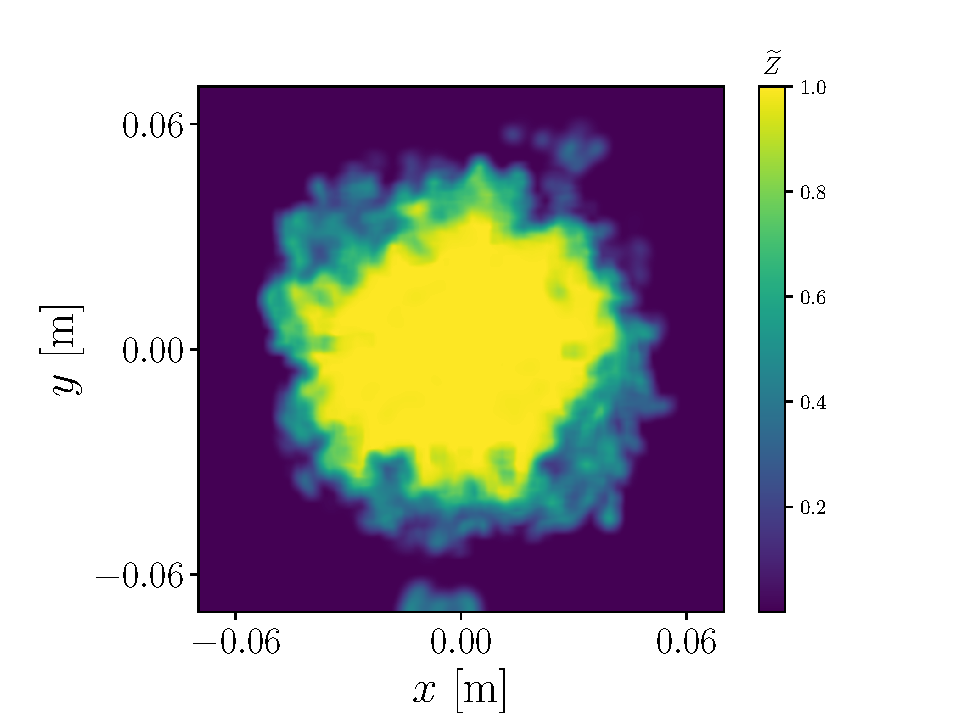
\includegraphics[page=1, width=0.2\textwidth]{./figs/dice_0002_slice.pdf}%
    \includegraphics[page=2, width=0.2\textwidth]{./figs/dice_0002_slice.pdf}%
    \includegraphics[page=3, width=0.2\textwidth]{./figs/dice_0002_slice.pdf}%
    \includegraphics[page=4, width=0.2\textwidth]{./figs/dice_0002_slice.pdf}%
    \includegraphics[page=5, width=0.2\textwidth]{./figs/dice_0002_slice.pdf}\\[1cm]%
    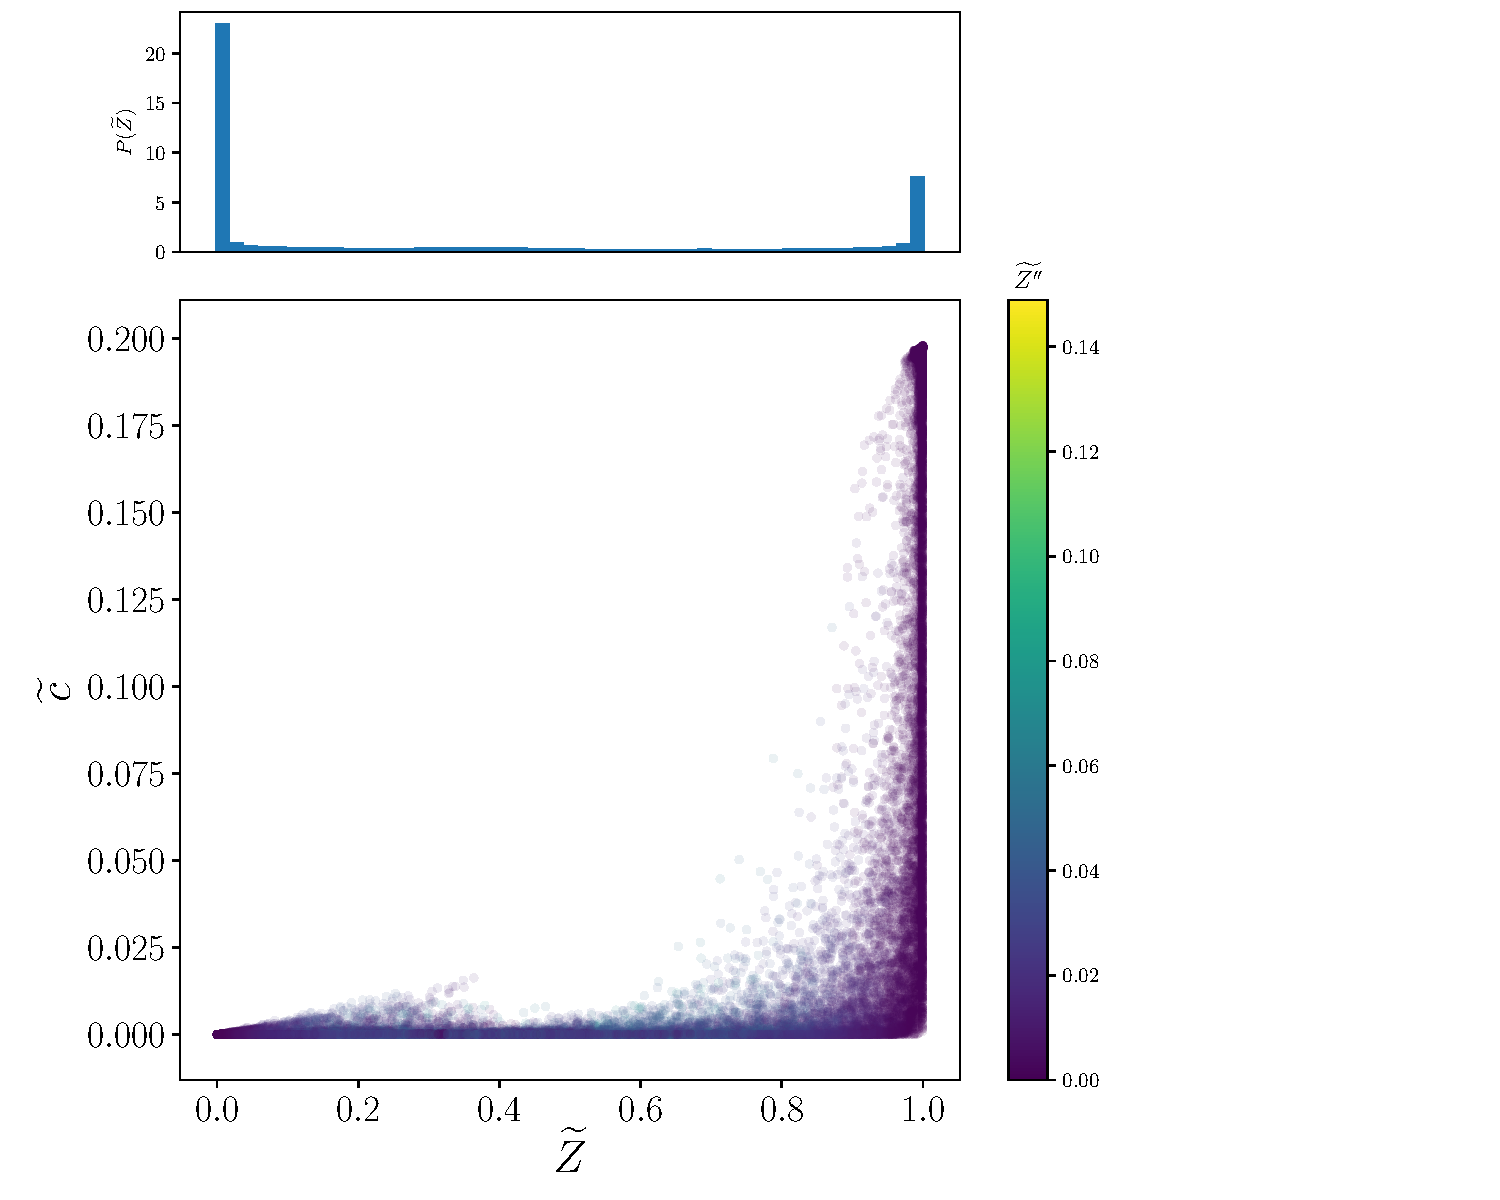
\includegraphics[page=1, height=0.3\textwidth, trim=0.0cm 0cm 6.4cm 0cm, clip]{./figs/inputs_dice_0002.pdf}%
    \includegraphics[page=2, height=0.3\textwidth, trim=1.0cm 0cm 2.4cm 0cm, clip]{./figs/inputs_dice_0002.pdf}%
    \includegraphics[page=3, height=0.3\textwidth, trim=0.0cm 0cm 2.4cm 0cm, clip]{./figs/inputs_dice_0002.pdf}%
  \end{figure}%
}
\frame{
  \frametitle{Dice 3: slices and PDF input space}
  \begin{figure}[!tbp]%
    \centering%
    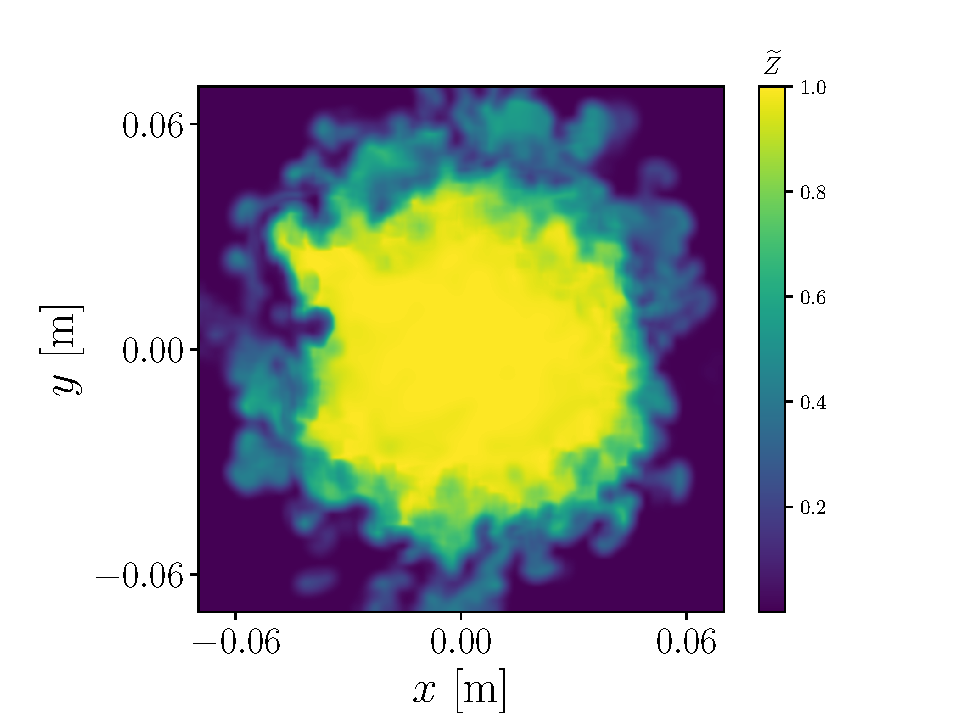
\includegraphics[page=1, width=0.2\textwidth]{./figs/dice_0003_slice.pdf}%
    \includegraphics[page=2, width=0.2\textwidth]{./figs/dice_0003_slice.pdf}%
    \includegraphics[page=3, width=0.2\textwidth]{./figs/dice_0003_slice.pdf}%
    \includegraphics[page=4, width=0.2\textwidth]{./figs/dice_0003_slice.pdf}%
    \includegraphics[page=5, width=0.2\textwidth]{./figs/dice_0003_slice.pdf}\\[1cm]%
    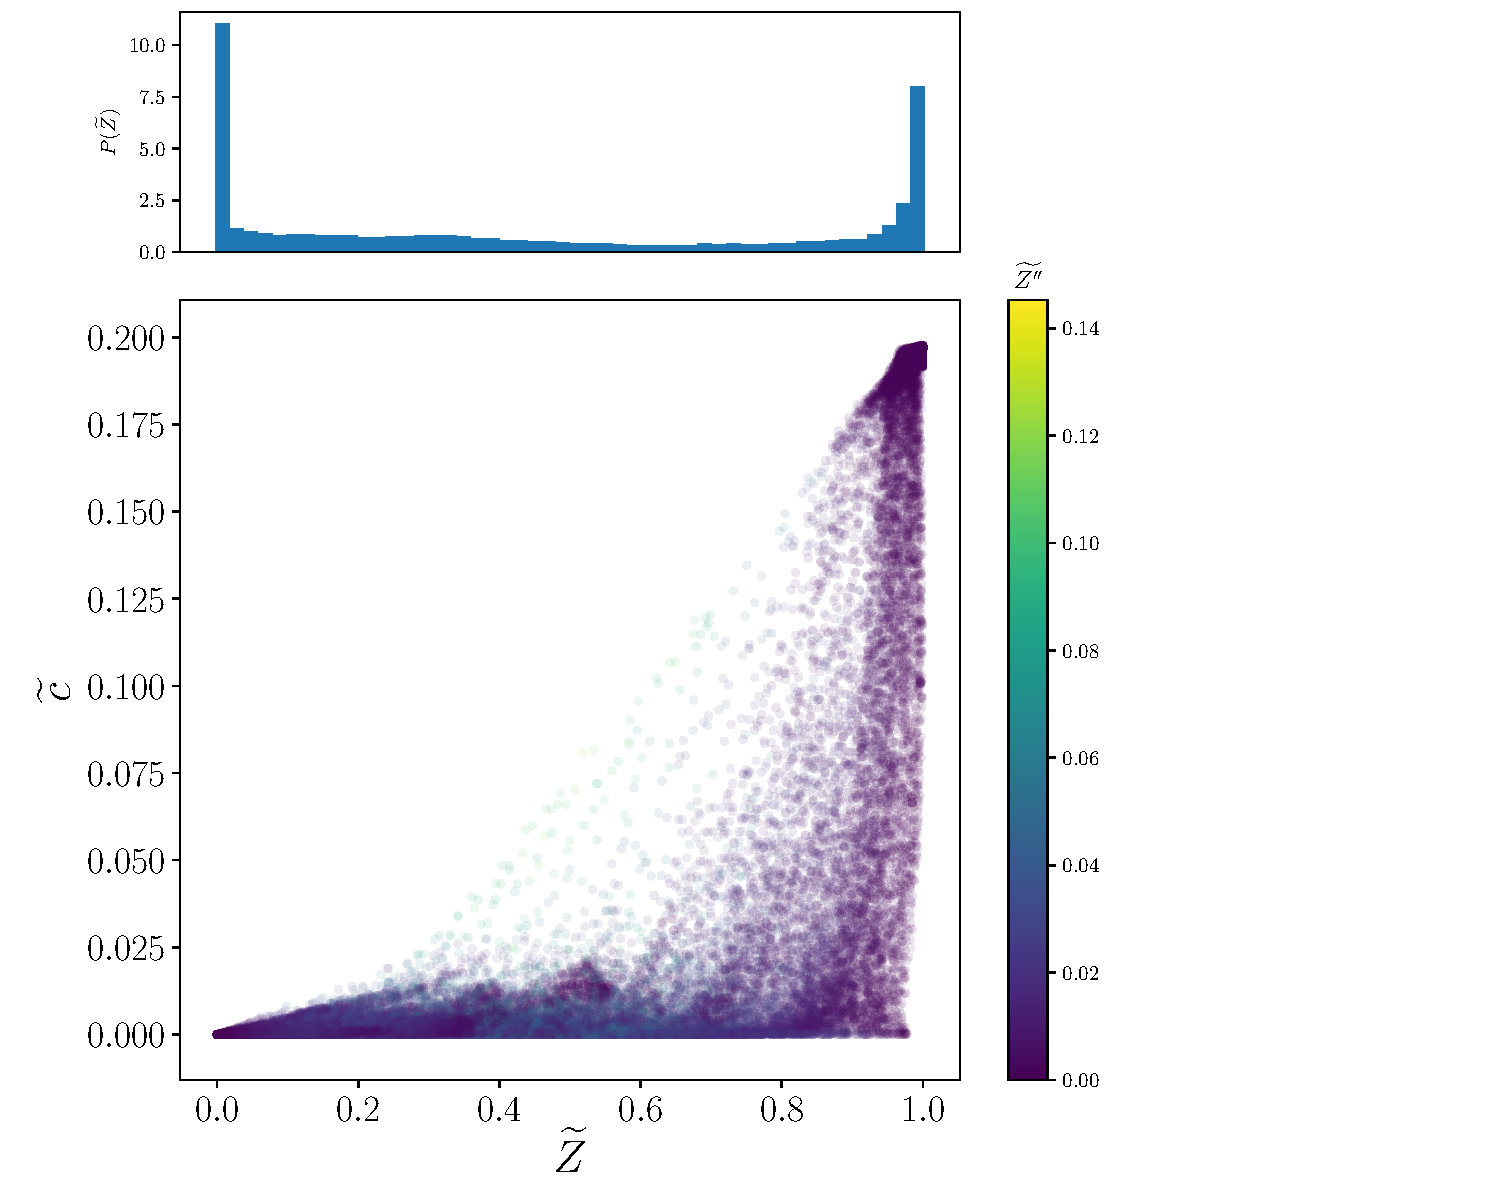
\includegraphics[page=1, height=0.3\textwidth, trim=0.0cm 0cm 6.4cm 0cm, clip]{./figs/inputs_dice_0003.pdf}%
    \includegraphics[page=2, height=0.3\textwidth, trim=1.0cm 0cm 2.4cm 0cm, clip]{./figs/inputs_dice_0003.pdf}%
    \includegraphics[page=3, height=0.3\textwidth, trim=0.0cm 0cm 2.4cm 0cm, clip]{./figs/inputs_dice_0003.pdf}%
  \end{figure}%
}
\frame{
  \frametitle{Dice 4: slices and PDF input space}
  \begin{figure}[!tbp]%
    \centering%
    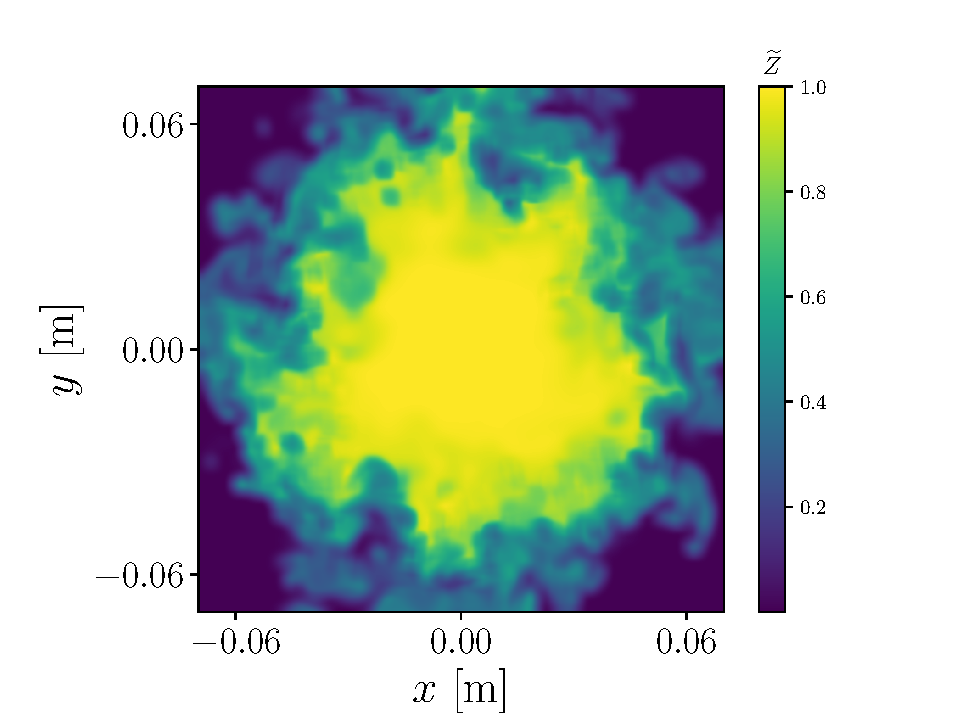
\includegraphics[page=1, width=0.2\textwidth]{./figs/dice_0004_slice.pdf}%
    \includegraphics[page=2, width=0.2\textwidth]{./figs/dice_0004_slice.pdf}%
    \includegraphics[page=3, width=0.2\textwidth]{./figs/dice_0004_slice.pdf}%
    \includegraphics[page=4, width=0.2\textwidth]{./figs/dice_0004_slice.pdf}%
    \includegraphics[page=5, width=0.2\textwidth]{./figs/dice_0004_slice.pdf}\\[1cm]%
    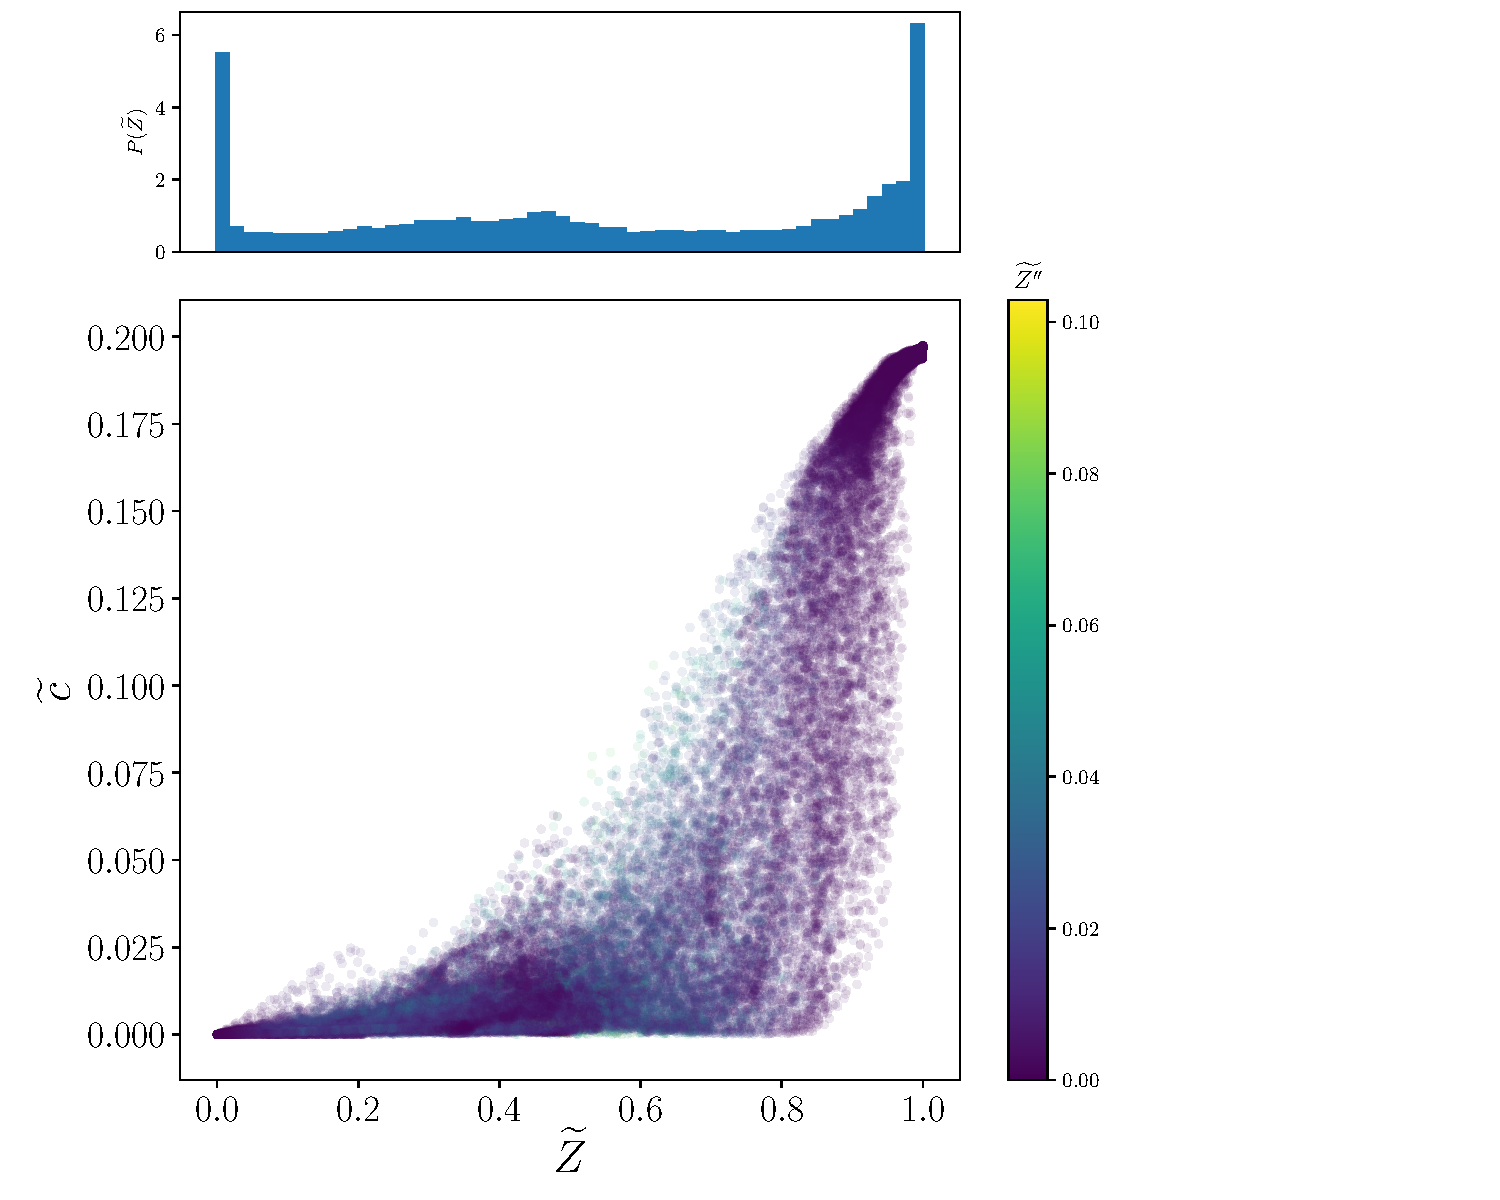
\includegraphics[page=1, height=0.3\textwidth, trim=0.0cm 0cm 6.4cm 0cm, clip]{./figs/inputs_dice_0004.pdf}%
    \includegraphics[page=2, height=0.3\textwidth, trim=1.0cm 0cm 2.4cm 0cm, clip]{./figs/inputs_dice_0004.pdf}%
    \includegraphics[page=3, height=0.3\textwidth, trim=0.0cm 0cm 2.4cm 0cm, clip]{./figs/inputs_dice_0004.pdf}%
  \end{figure}%
}
\frame{
  \frametitle{Dice 5: slices and PDF input space}
  \begin{figure}[!tbp]%
    \centering%
    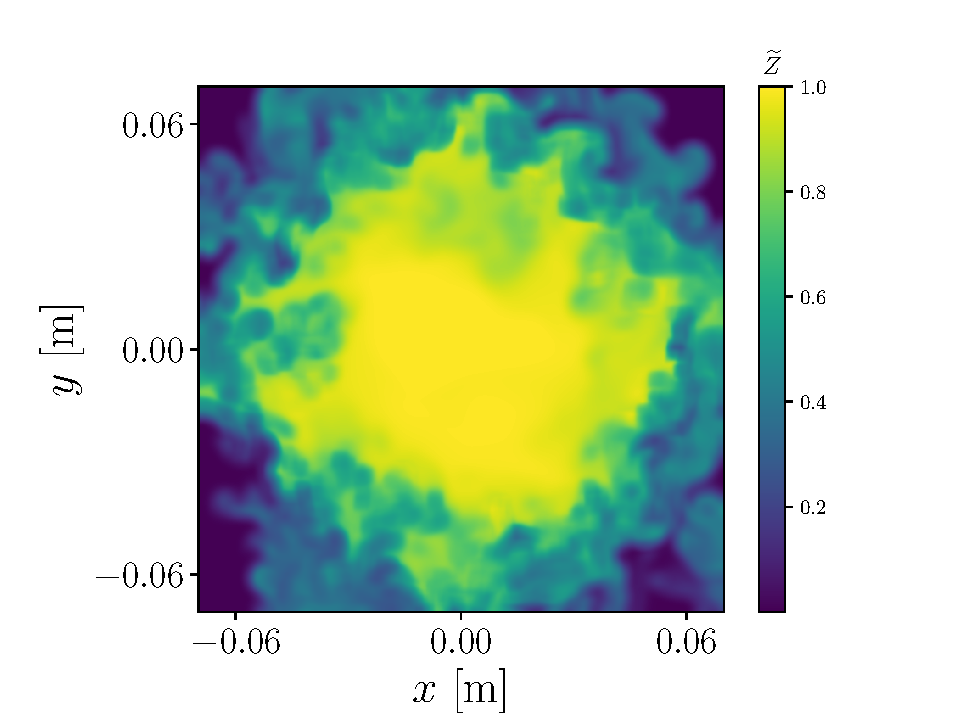
\includegraphics[page=1, width=0.2\textwidth]{./figs/dice_0005_slice.pdf}%
    \includegraphics[page=2, width=0.2\textwidth]{./figs/dice_0005_slice.pdf}%
    \includegraphics[page=3, width=0.2\textwidth]{./figs/dice_0005_slice.pdf}%
    \includegraphics[page=4, width=0.2\textwidth]{./figs/dice_0005_slice.pdf}%
    \includegraphics[page=5, width=0.2\textwidth]{./figs/dice_0005_slice.pdf}\\[1cm]%
    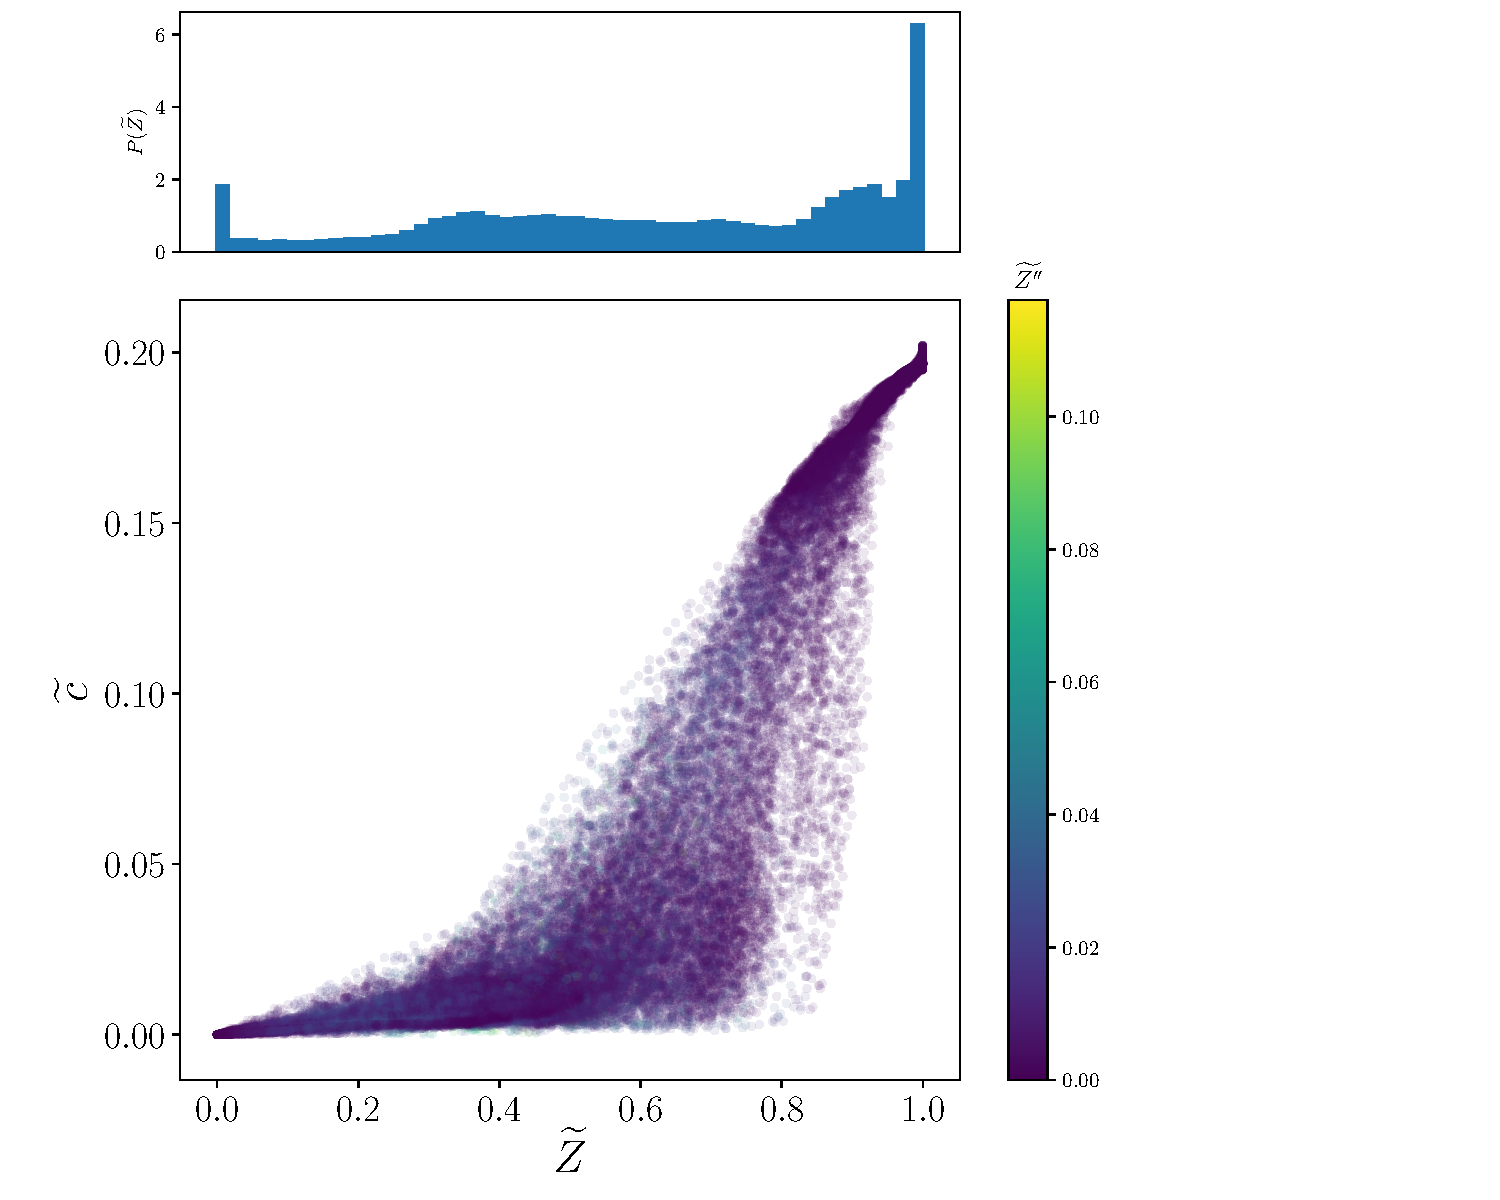
\includegraphics[page=1, height=0.3\textwidth, trim=0.0cm 0cm 6.4cm 0cm, clip]{./figs/inputs_dice_0005.pdf}%
    \includegraphics[page=2, height=0.3\textwidth, trim=1.0cm 0cm 2.4cm 0cm, clip]{./figs/inputs_dice_0005.pdf}%
    \includegraphics[page=3, height=0.3\textwidth, trim=0.0cm 0cm 2.4cm 0cm, clip]{./figs/inputs_dice_0005.pdf}%
  \end{figure}%
}
\frame{
  \frametitle{Dice 6: slices and PDF input space}
  \begin{figure}[!tbp]%
    \centering%
    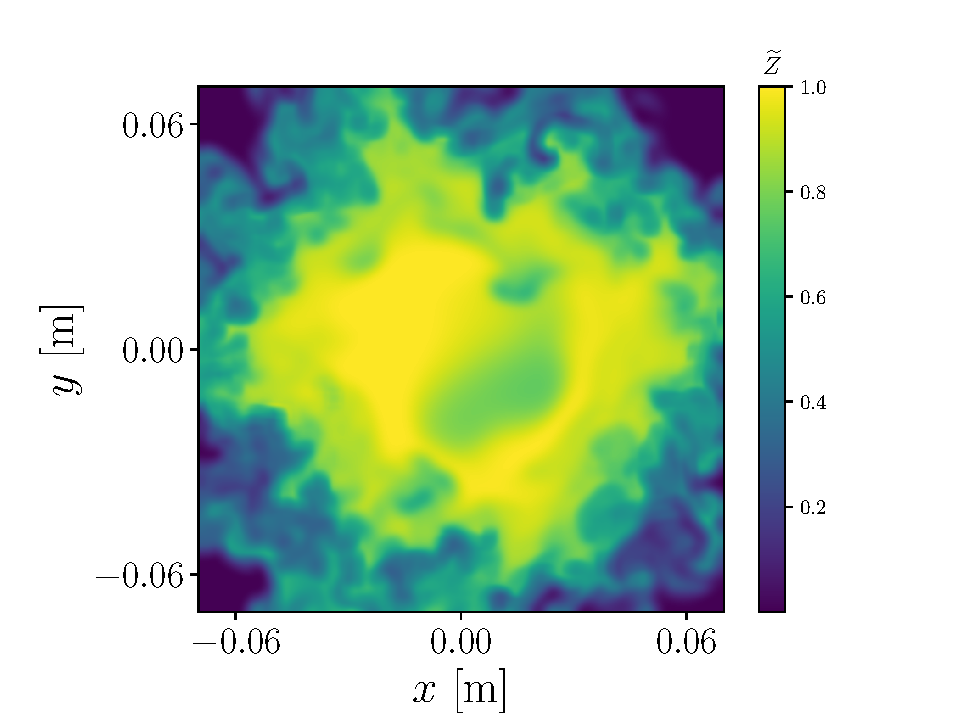
\includegraphics[page=1, width=0.2\textwidth]{./figs/dice_0006_slice.pdf}%
    \includegraphics[page=2, width=0.2\textwidth]{./figs/dice_0006_slice.pdf}%
    \includegraphics[page=3, width=0.2\textwidth]{./figs/dice_0006_slice.pdf}%
    \includegraphics[page=4, width=0.2\textwidth]{./figs/dice_0006_slice.pdf}%
    \includegraphics[page=5, width=0.2\textwidth]{./figs/dice_0006_slice.pdf}\\[1cm]%
    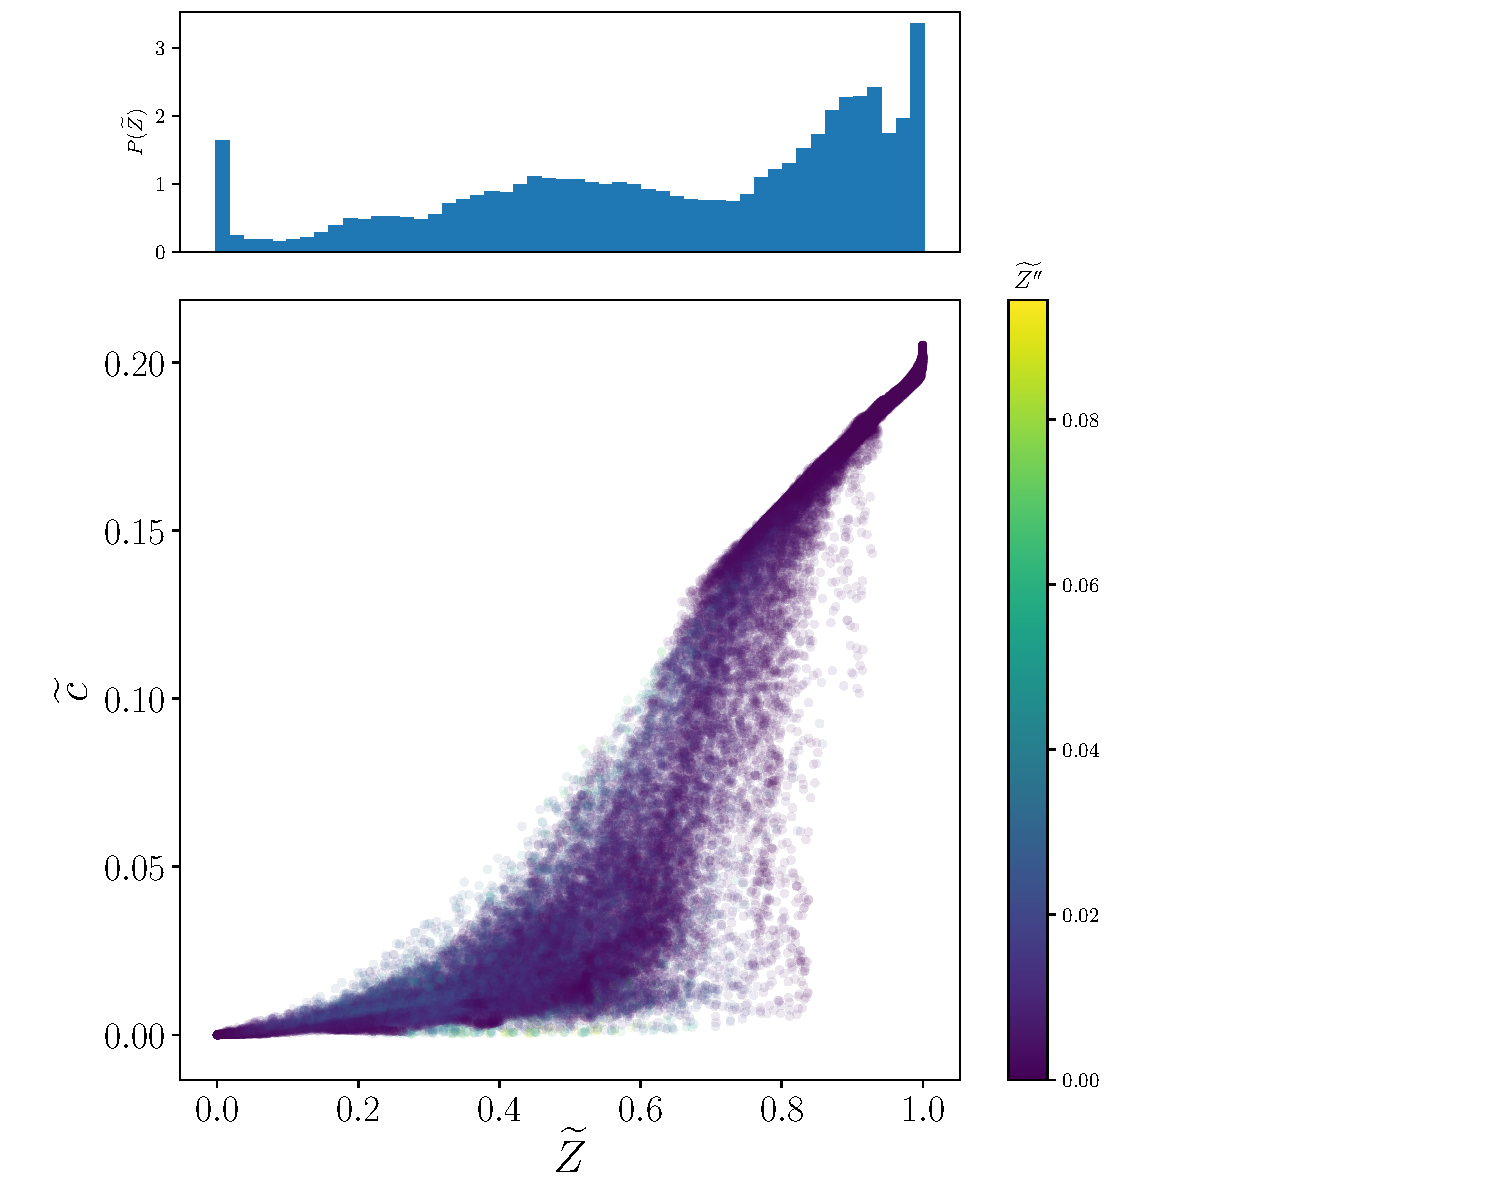
\includegraphics[page=1, height=0.3\textwidth, trim=0.0cm 0cm 6.4cm 0cm, clip]{./figs/inputs_dice_0006.pdf}%
    \includegraphics[page=2, height=0.3\textwidth, trim=1.0cm 0cm 2.4cm 0cm, clip]{./figs/inputs_dice_0006.pdf}%
    \includegraphics[page=3, height=0.3\textwidth, trim=0.0cm 0cm 2.4cm 0cm, clip]{./figs/inputs_dice_0006.pdf}%
  \end{figure}%
}
\frame{
  \frametitle{Dice 7: slices and PDF input space}
  \begin{figure}[!tbp]%
    \centering%
    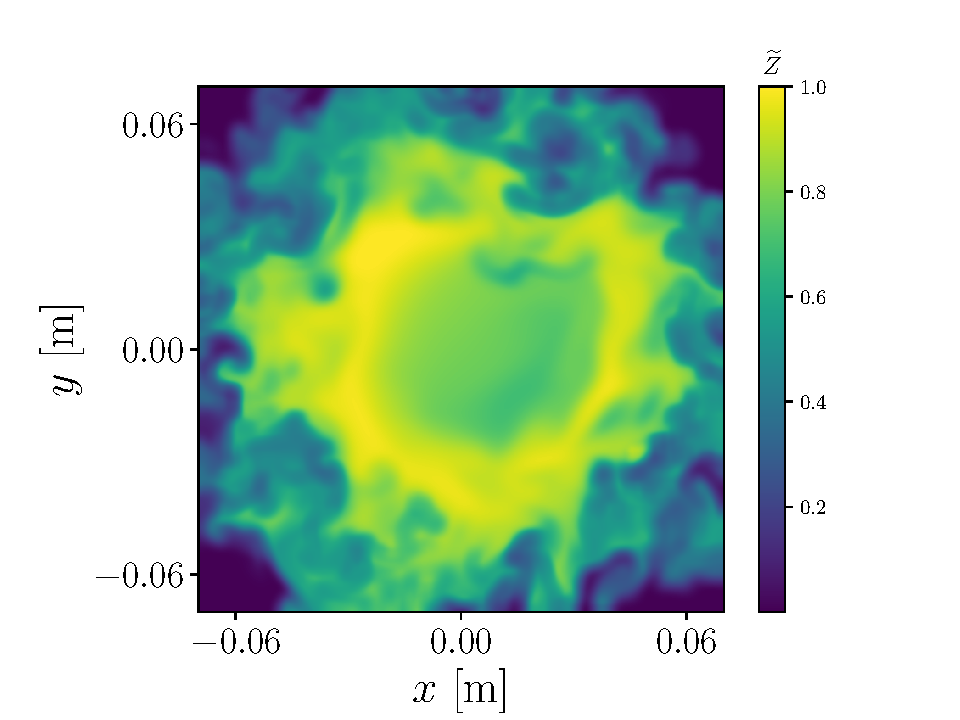
\includegraphics[page=1, width=0.2\textwidth]{./figs/dice_0007_slice.pdf}%
    \includegraphics[page=2, width=0.2\textwidth]{./figs/dice_0007_slice.pdf}%
    \includegraphics[page=3, width=0.2\textwidth]{./figs/dice_0007_slice.pdf}%
    \includegraphics[page=4, width=0.2\textwidth]{./figs/dice_0007_slice.pdf}%
    \includegraphics[page=5, width=0.2\textwidth]{./figs/dice_0007_slice.pdf}\\[1cm]%
    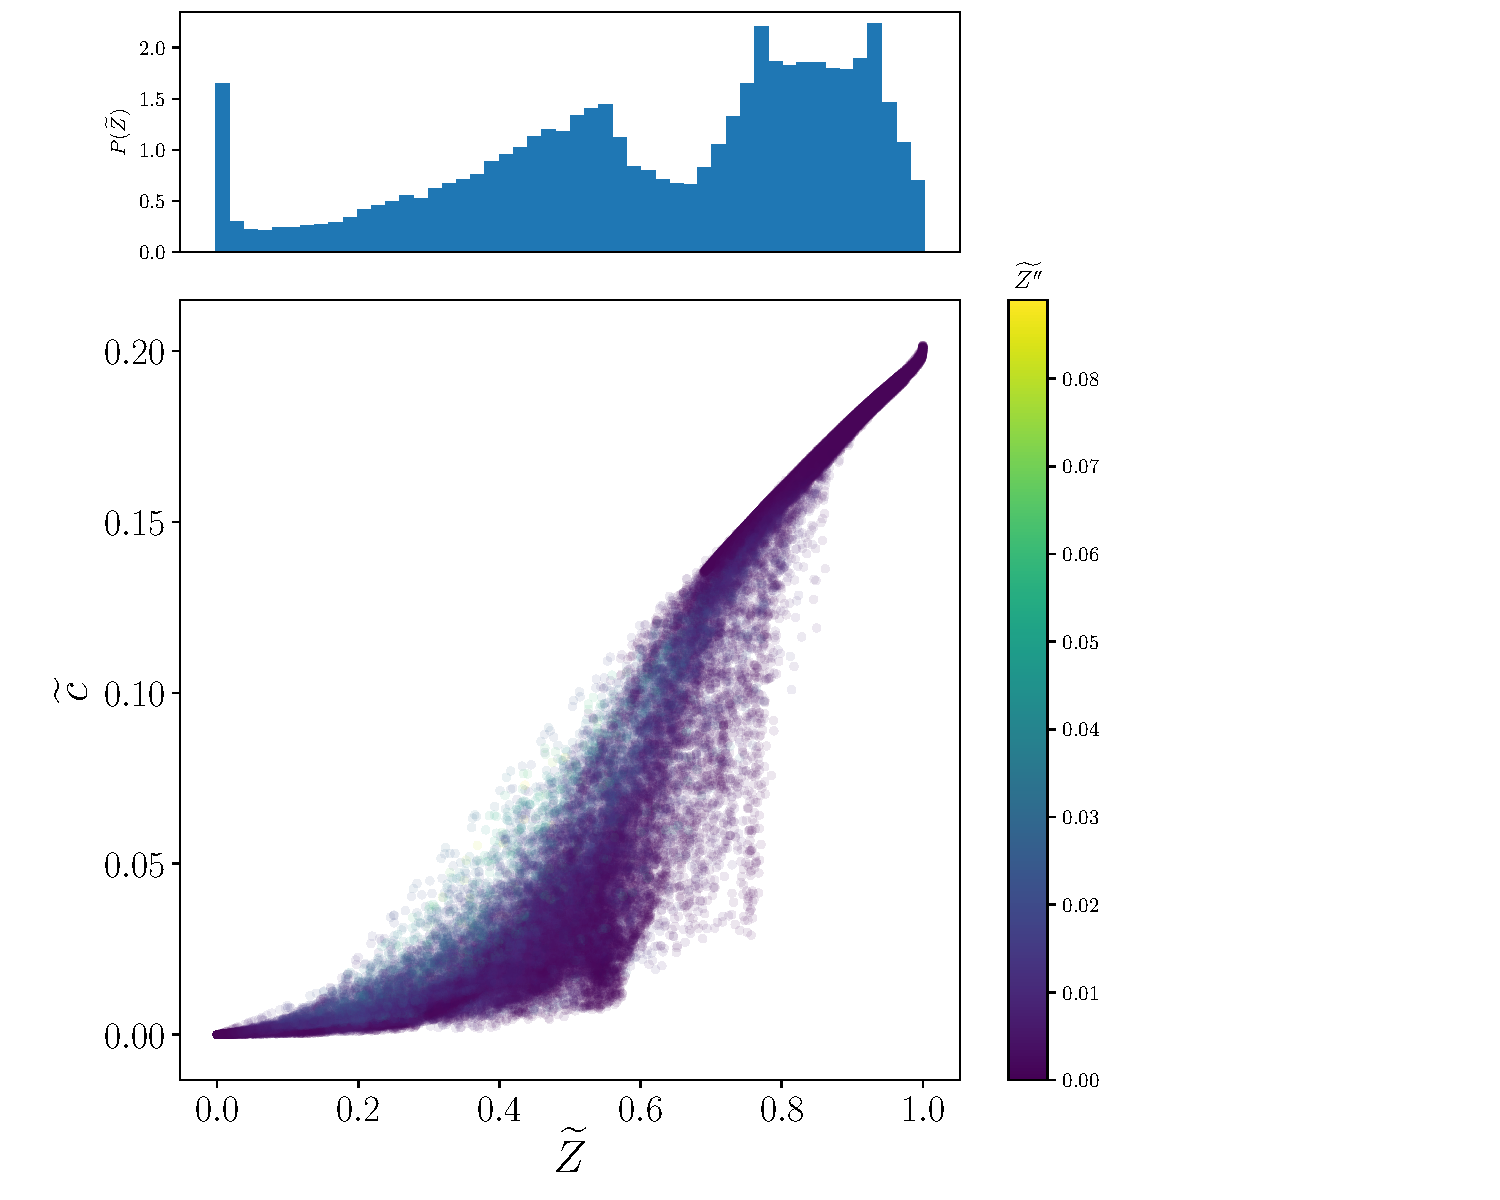
\includegraphics[page=1, height=0.3\textwidth, trim=0.0cm 0cm 6.4cm 0cm, clip]{./figs/inputs_dice_0007.pdf}%
    \includegraphics[page=2, height=0.3\textwidth, trim=1.0cm 0cm 2.4cm 0cm, clip]{./figs/inputs_dice_0007.pdf}%
    \includegraphics[page=3, height=0.3\textwidth, trim=0.0cm 0cm 2.4cm 0cm, clip]{./figs/inputs_dice_0007.pdf}%
  \end{figure}%
}
\frame{
  \frametitle{Dice 8: slices and PDF input space}
  \begin{figure}[!tbp]%
    \centering%
    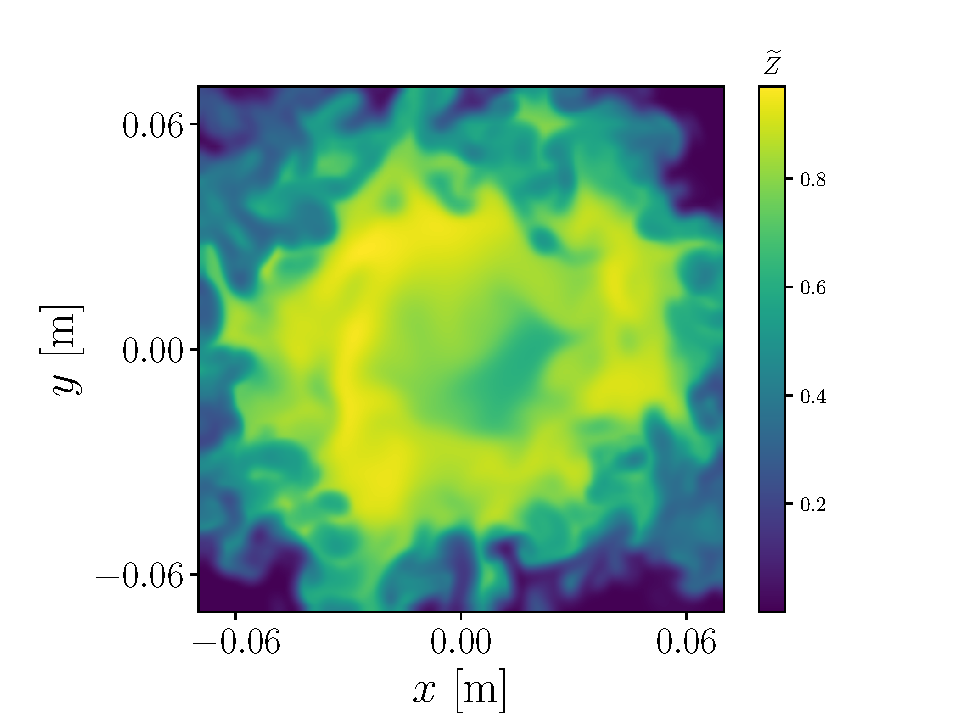
\includegraphics[page=1, width=0.2\textwidth]{./figs/dice_0008_slice.pdf}%
    \includegraphics[page=2, width=0.2\textwidth]{./figs/dice_0008_slice.pdf}%
    \includegraphics[page=3, width=0.2\textwidth]{./figs/dice_0008_slice.pdf}%
    \includegraphics[page=4, width=0.2\textwidth]{./figs/dice_0008_slice.pdf}%
    \includegraphics[page=5, width=0.2\textwidth]{./figs/dice_0008_slice.pdf}\\[1cm]%
    \includegraphics[page=1, height=0.3\textwidth, trim=0.0cm 0cm 6.4cm 0cm, clip]{./figs/inputs_dice_0008.pdf}%
    \includegraphics[page=2, height=0.3\textwidth, trim=1.0cm 0cm 2.4cm 0cm, clip]{./figs/inputs_dice_0008.pdf}%
    \includegraphics[page=3, height=0.3\textwidth, trim=0.0cm 0cm 2.4cm 0cm, clip]{./figs/inputs_dice_0008.pdf}%
  \end{figure}%
}
\frame{
  \frametitle{Dice 9: slices and PDF input space}
  \begin{figure}[!tbp]%
    \centering%
    \includegraphics[page=1, width=0.2\textwidth]{./figs/dice_0009_slice.pdf}%
    \includegraphics[page=2, width=0.2\textwidth]{./figs/dice_0009_slice.pdf}%
    \includegraphics[page=3, width=0.2\textwidth]{./figs/dice_0009_slice.pdf}%
    \includegraphics[page=4, width=0.2\textwidth]{./figs/dice_0009_slice.pdf}%
    \includegraphics[page=5, width=0.2\textwidth]{./figs/dice_0009_slice.pdf}\\[1cm]%
    \includegraphics[page=1, height=0.3\textwidth, trim=0.0cm 0cm 6.4cm 0cm, clip]{./figs/inputs_dice_0009.pdf}%
    \includegraphics[page=2, height=0.3\textwidth, trim=1.0cm 0cm 2.4cm 0cm, clip]{./figs/inputs_dice_0009.pdf}%
    \includegraphics[page=3, height=0.3\textwidth, trim=0.0cm 0cm 2.4cm 0cm, clip]{./figs/inputs_dice_0009.pdf}%
  \end{figure}%
}
\frame{
  \frametitle{Dice 10: slices and PDF input space}
  \begin{figure}[!tbp]%
    \centering%
    \includegraphics[page=1, width=0.2\textwidth]{./figs/dice_0010_slice.pdf}%
    \includegraphics[page=2, width=0.2\textwidth]{./figs/dice_0010_slice.pdf}%
    \includegraphics[page=3, width=0.2\textwidth]{./figs/dice_0010_slice.pdf}%
    \includegraphics[page=4, width=0.2\textwidth]{./figs/dice_0010_slice.pdf}%
    \includegraphics[page=5, width=0.2\textwidth]{./figs/dice_0010_slice.pdf}\\[1cm]%
    \includegraphics[page=1, height=0.3\textwidth, trim=0.0cm 0cm 6.4cm 0cm, clip]{./figs/inputs_dice_0010.pdf}%
    \includegraphics[page=2, height=0.3\textwidth, trim=1.0cm 0cm 2.4cm 0cm, clip]{./figs/inputs_dice_0010.pdf}%
    \includegraphics[page=3, height=0.3\textwidth, trim=0.0cm 0cm 2.4cm 0cm, clip]{./figs/inputs_dice_0010.pdf}%
  \end{figure}%
}

\frame{
  \frametitle{Convolution prediction}
  \begin{align*}
    \langle \wt{\dot{\omega}} | \wt{Z}, \wt{Z''}, \wt{C}, \wt{C''}\rangle = \int \langle \dot{\omega} | Z, C \rangle P(Z,C | \wt{Z}, \wt{Z''}, \wt{C}, \wt{C''}) \ud Z \ud C
  \end{align*}
  where $\langle \wt{\dot{\omega}} | \wt{Z}, \wt{Z''}, \wt{C}, \wt{C''}\rangle$, $\langle \dot{\omega} | Z, C \rangle$, $P(Z,C | \wt{Z}, \wt{Z''}, \wt{C}, \wt{C''})$\newline
  are from the same $32^3$ block
}
{
  \setbeamercolor{background canvas}{bg=}
  \includepdf[pages={1,2}]{./figs/convolution_exact.pdf}
}

%=================================================================================
% RF and results
\section{Regression models with machine learning}\label{sec:ml}
\subsection{Random forest}\label{sec:RF}
\begin{frame}[fragile]
  \frametitle{ML \#1: Random Forest, 100 trees, max depth of 30}
  {\small \verbatiminput{./figs/RF.log}}
\end{frame}

{
  \setbeamercolor{background canvas}{bg=}
  \includepdf[pages={1}]{./figs/RF.pdf}
  \includepdf[pages={2,3}]{./figs/RF.pdf}
}

\frame{
  \frametitle{Convolution prediction}
}
{
  \setbeamercolor{background canvas}{bg=}
  \includepdf[pages={1,2}]{./figs/convolution_RF.pdf}
}

%=================================================================================
% LR and results
\subsection{Linear regression}\label{sec:LR}
\begin{frame}[fragile]
  \frametitle{ML \#2: Linear regression (clipped and normalized)}
  {\small \verbatiminput{./figs/LR.log}}
\end{frame}

% results
{
  \setbeamercolor{background canvas}{bg=}
  \includepdf[pages={1}]{./figs/LR.pdf}
  \includepdf[pages={2,3}]{./figs/LR.pdf}
}

% =================================================================================
% PR and results
\subsection{Polynomial regression}\label{sec:PR}
\begin{frame}[fragile]
  \frametitle{ML \#3: Polynomial regression (clipped and normalized)}
  \only<1>{\small Order 1:\vspace{-0.4cm} \verbatiminput{./figs/LR.log}}
  \only<2>{\small Order 2:\vspace{-0.4cm} \verbatiminput{./figs/PR2.log}}
  \only<3>{\small Order 3:\vspace{-0.4cm} \verbatiminput{./figs/PR3.log}}
  \only<4>{\small Order 6:\vspace{-0.4cm} \verbatiminput{./figs/PR6.log}}
\end{frame}

% results for PR6
{
  \setbeamercolor{background canvas}{bg=}
  \includepdf[pages={1}]{./figs/PR6.pdf}
  \includepdf[pages={2,3}]{./figs/PR6.pdf}
}

\frame{
  \frametitle{Convolution prediction}
}
{
  \setbeamercolor{background canvas}{bg=}
  \includepdf[pages={1,2}]{./figs/convolution_PR6.pdf}
}


%=================================================================================
% DNN and results
\subsection{DNN}\label{sec:DNN}
\begin{frame}[fragile]
  \frametitle{ML \#4: DNN, $[256,512,2048]$ nodes, BCEloss, $l = 10^{-4}$}
  {\small \verbatiminput{./figs/DNN.log}}
\end{frame}

{
  \setbeamercolor{background canvas}{bg=}
  \includepdf[pages={1}]{./figs/DNN.pdf}
  \includepdf[pages={2,3}]{./figs/DNN.pdf}
}

\frame{
  \frametitle{Convolution prediction}
}
{
  \setbeamercolor{background canvas}{bg=}
  \includepdf[pages={1,2}]{./figs/convolution_DNN.pdf}
}

%=================================================================================
% CVAE and results
\section[Generative models]{Generative models}\label{sec:gm}
\subsection{Conditional Variational Autoencoder}\label{sec:CVAE}
\begin{frame}[fragile]
  \frametitle{GM \#1: CVAE}
  {\small \verbatiminput{./figs/CVAE.log}}
\end{frame}

{
  \setbeamercolor{background canvas}{bg=}
  \includepdf[pages={1}]{./figs/CVAE.pdf}
  \includepdf[pages={2,3}]{./figs/CVAE.pdf}
}

\frame{
  \frametitle{Convolution prediction}
}
{
  \setbeamercolor{background canvas}{bg=}
  \includepdf[pages={1,2}]{./figs/convolution_CVAE.pdf}
}

%=================================================================================
% CGAN and results
\subsection{Conditional Generative Adversarial Network}\label{sec:CGAN}
\begin{frame}[fragile]
  \frametitle{GM \#2: CGAN}
  {\small \verbatiminput{./figs/CGAN.log}}
\end{frame}

{
  \setbeamercolor{background canvas}{bg=}
  \includepdf[pages={1}]{./figs/CGAN.pdf}
  \includepdf[pages={2,3}]{./figs/CGAN.pdf}
}

\frame{
  \frametitle{Convolution prediction}
}
{
  \setbeamercolor{background canvas}{bg=}
  \includepdf[pages={1,2}]{./figs/convolution_CGAN.pdf}
}

%=================================================================================
% delta-delta and results
\section{Physics models}\label{sec:physics}
\subsection{$\delta-\delta$ model}\label{sec:DD}
\begin{frame}[fragile]
  \frametitle{Physics \#1: $\delta-\delta$ PDF}
  {\small \verbatiminput{./figs/DD.log}}
\end{frame}

{
  \setbeamercolor{background canvas}{bg=}
  \includepdf[pages={1}]{./figs/DD.pdf}
  \includepdf[pages={2,3}]{./figs/DD.pdf}
}

\frame{
  \frametitle{Convolution prediction}
}
{
  \setbeamercolor{background canvas}{bg=}
  \includepdf[pages={1,2}]{./figs/convolution_DD.pdf}
}

%=================================================================================
% beta-delta and results
\subsection{$\beta-\delta$ model}\label{sec:BD}
\begin{frame}[fragile]
  \frametitle{Physics \#2: $\beta(Z)-\delta(C)$ PDF}
  {\small \verbatiminput{./figs/BD.log}}
\end{frame}

{
  \setbeamercolor{background canvas}{bg=}
  \includepdf[pages={1}]{./figs/BD.pdf}
  \includepdf[pages={2,3}]{./figs/BD.pdf}
}

\frame{
  \frametitle{Convolution prediction}
}
{
  \setbeamercolor{background canvas}{bg=}
  \includepdf[pages={1,2}]{./figs/convolution_BD.pdf}
}

%=================================================================================
% beta-beta and results
\subsection{$\beta-\beta$ model}\label{sec:BB}
\begin{frame}[fragile]
  \frametitle{Physics \#3: $\beta(Z)-\beta(C)$ PDF}
  {\small \verbatiminput{./figs/BB.log}}
\end{frame}

{
  \setbeamercolor{background canvas}{bg=}
  \includepdf[pages={1}]{./figs/BB.pdf}
  \includepdf[pages={2,3}]{./figs/BB.pdf}
}

\frame{
  \frametitle{Convolution prediction}
}
{
  \setbeamercolor{background canvas}{bg=}
  \includepdf[pages={1,2}]{./figs/convolution_BB.pdf}
}

%=================================================================================
% timings
\section{Summary}\label{sec:summary}
\frame{
  \frametitle{Model performance summary}
  \begin{table}[]
    \begin{tabular}{lccccc}
      \toprule
      model & $J_{90}$ & Prediction time (s) & RMSE for $\widetilde{\dot{\omega}}$ & $R^2$ for $\widetilde{\dot{\omega}}$ & Size (MB)\\
      \midrule
      RF            & 0.12 & 2.75 & 0.4  &  0.96 & 82149 \\
      DNN           & 0.11 & 0.15 & 0.35 &  0.97 & 27    \\
      CVAE          & 0.12 & 0.11 & 0.34 &  0.97 & 36    \\
      $\beta-\beta$ & 0.33 & {--} & 1.05 &  0.7  & {--}  \\
      \bottomrule
    \end{tabular}
  \end{table}
}

%=================================================================================
% generalization
\section{Generalization}\label{sec:generalization}
\frame{
  \frametitle{Predicting on other dices}
  \tiny

  % RF
  \setbeamercolor{coloredbox}{fg=black,bg=c2med}
  \begin{beamercolorbox}[wd=\textwidth,sep=1ex]{coloredbox}
    \centering
    RF
  \end{beamercolorbox}
  \begin{minipage}{.3\linewidth}
    \centering
    Trained on dice 2\\[0.1cm]
    \begin{tabular}{ccc}
      dice & JSD 90 & RMSE\\
      \hline
      1 & 0.225506 & 2.546500 \\
      2 & 0.121005 & 0.398052 \\
      3 & 0.311023 & 0.302434 \\
      4 & 0.540858 & 0.247165 \\
      5 & 0.637645 & 0.189663
    \end{tabular}
  \end{minipage}\hfill%
  \begin{minipage}{.3\linewidth}
    \centering
    Trained on dice 3\\[0.1cm]
    \begin{tabular}{ccc}
      dice & JSD 90 & RMSE\\
      \hline
      1 & 0.471538 & 14.606095 \\
      2 & 0.212643 &  2.163460 \\
      3 & 0.151371 &  0.165814 \\
      4 & 0.304312 &  0.149800 \\
      5 & 0.513507 &  0.117921
    \end{tabular}
  \end{minipage}\hfill
  \begin{minipage}{.3\linewidth}
    \centering
    Trained on all dices\\[0.1cm]
    \begin{tabular}{ccc}
      dice & JSD 90 & RMSE\\
      \hline
      1 & 0.038393 & 0.319048 \\
      2 & 0.119613 & 0.351820 \\
      3 & 0.179026 & 0.155962 \\
      4 & 0.211864 & 0.096622 \\
      5 & 0.251139 & 0.082761
    \end{tabular}
  \end{minipage}\\[0.3cm]

  % DNN
  \begin{beamercolorbox}[wd=\textwidth,sep=1ex]{coloredbox}
    \centering
    DNN
  \end{beamercolorbox}
  \begin{minipage}{.3\linewidth}
    \centering
    Trained on dice 2\\[0.1cm]
    \begin{tabular}{ccc}
      dice & JSD 90 & RMSE\\
      \hline
      1 & 0.302302 & 1.511685 \\
      2 & 0.113093 & 0.352330 \\
      3 & 0.269360 & 0.267391 \\
      4 & 0.523166 & 0.204584 \\
      5 & 0.586430 & 0.154679
    \end{tabular}
  \end{minipage}\hfill%
  \begin{minipage}{.3\linewidth}
    \centering
    Trained on dice 3\\[0.1cm]
    \begin{tabular}{ccc}
      dice & JSD 90 & RMSE\\
      \hline
      1 & 0.638801 & 4.430153 \\
      2 & 0.221772 & 0.997562 \\
      3 & 0.145944 & 0.185941 \\
      4 & 0.283154 & 0.132489 \\
      5 & 0.466592 & 0.101539
    \end{tabular}
  \end{minipage}\hfill
  \begin{minipage}{.3\linewidth}
    \centering
    Trained on all dices\\[0.1cm]
    \begin{tabular}{ccc}
      dice & JSD 90 & RMSE\\
      \hline
      1 & 0.051776 & 0.538867\\
      2 & 0.122495 & 0.369603\\
      3 & 0.164724 & 0.173918\\
      4 & 0.184673 & 0.104286\\
      5 & 0.223159 & 0.080714
    \end{tabular}
  \end{minipage}\\[0.3cm]

  % CVAE
  \setbeamercolor{coloredbox}{fg=black,bg=c2med}
  \begin{beamercolorbox}[wd=\textwidth,sep=1ex]{coloredbox}
    \centering
    CVAE
  \end{beamercolorbox}
  \begin{minipage}{.3\linewidth}
    \centering
    Trained on dice 2\\[0.1cm]
    \begin{tabular}{ccc}
      dice & JSD 90 & RMSE\\
      \hline
      1 & 0.266282 & 1.527464 \\
      2 & 0.116341 & 0.344944 \\
      3 & 0.334746 & 0.324995 \\
      4 & 0.693120 & 0.236547 \\
      5 & 0.693147 & 0.173310
    \end{tabular}
  \end{minipage}\hfill%
  \begin{minipage}{.3\linewidth}
    \centering
    Trained on dice 3\\[0.1cm]
    \begin{tabular}{ccc}
      dice & JSD 90 & RMSE\\
      \hline
      1 &  0.667684 & 8.935289 \\
      2 &  0.244925 & 1.212532 \\
      3 &  0.142852 & 0.169246 \\
      4 &  0.350593 & 0.144737 \\
      5 &  0.641043 & 0.108570
    \end{tabular}
  \end{minipage}\hfill
  \begin{minipage}{.3\linewidth}
    \centering
    Trained on all dices\\[0.1cm]
    \begin{tabular}{ccc}
      dice & JSD 90 & RMSE\\
      \hline
      1 &  0.053327 & 0.427858 \\
      2 &  0.122943 & 0.391131 \\
      3 &  0.157860 & 0.172827 \\
      4 &  0.176537 & 0.101066 \\
      5 &  0.214239 & 0.079102
    \end{tabular}
  \end{minipage}
}

\frame{
  \frametitle{Predicting on other dices}
  \tiny

  % BB
  \setbeamercolor{coloredbox}{fg=black,bg=c2med}
  \begin{beamercolorbox}[wd=\textwidth,sep=1ex]{coloredbox}
    \centering
    BB
  \end{beamercolorbox}
  \hfill
  \begin{minipage}{.3\linewidth}
    \centering
    \begin{tabular}{ccc}
      dice & JSD 90 & RMSE\\
      \hline
      1 & 0.129426 & 1.312838 \\
      2 & 0.326514 & 1.044414 \\
      3 & 0.417348 & 0.522793 \\
      4 & 0.456653 & 0.261347 \\
      5 & 0.515507 & 0.180005
    \end{tabular}
  \end{minipage}
}

%=================================================================================
% conclusions
\section{Conclusions}\label{sec:ccl}
\frame{
  \frametitle{Conclusions}
  \structure{PDFs are complex in general}\\
  \hspace{1cm}ML does a good job of capturing complexity\\
  \hspace{1cm}Analytical models fail to capture complexity\\[0.3cm]
  \structure{Deep learning algorithms have an advantage in CFD-HPC}\\
  \hspace{1cm}high accuracy\\
  \hspace{1cm}fast prediction\\
  \hspace{1cm}better generalization\\[0.3cm]
  \structure{Generative algorithms not much of an advantage in this case}\\
  \hspace{1cm}very similar to DNN\\
  \hspace{1cm}provide ``realizations'' of PDFs
}

% % =================================================================================
% % Bibliography
% \begin{frame}[allowframebreaks,plain]{Bibliography}
%   \tiny
%   \bibliographystyle{model1-num-names}
%   %\bibliographystyle{jap}
%   \bibliography{./library}
% \end{frame}

% \egroup

\end{document}
